% Source for the figure of the partition of vectorQuickSort() in place
% (sec. 12.10): the keys written below and above the pivot at the two
% ends, the free places, and the next block read from the end with fewer
% free places. Build: make figures (in ../build).
\documentclass[border=4pt]{standalone}
\usepackage[T1]{fontenc}
\usepackage{lmodern}
\usepackage{amsmath,amssymb}
\usepackage{tikz}
\usepackage{lamalunga}
% tikz-ads.tex: the TikZ styles shared by the figures of the memory of the
% manual, \input by each standalone figure: a cell of a vector (cell), the
% cell that an operation touches (touched), a free cell (free), a node of a
% linked structure (node), the labels of indices (index) and of variables
% (var), a pointer (ptr), and \cells and \indices to draw a row of cells.
\usetikzlibrary{arrows.meta,positioning,calc,fit,shapes.multipart}
\definecolor{adsTouched}{RGB}{214,196,236}
\definecolor{adsFree}{RGB}{236,236,236}
\tikzset{
  ads/.style={>={Stealth[length=2mm]},font=\small,
              every node/.append style={inner sep=0pt}},
  cell/.style={draw,minimum width=7mm,minimum height=7mm,
               font=\small\ttfamily,outer sep=0pt},
  touched/.style={cell,fill=adsTouched},
  free/.style={cell,fill=adsFree,text=black!45},
  node/.style={draw,rounded corners=1pt,minimum width=8mm,
               minimum height=6mm,font=\small\ttfamily},
  index/.style={font=\scriptsize\ttfamily,text=black!60},
  var/.style={font=\small\itshape},
  ptr/.style={->,thick}
}
% \cells{name}{x,y}{list}: a row of cells, the first at (x,y), named
% name-0, name-1, ...; each item is text/style, the style one of cell,
% touched and free (e.g., {a/cell,e/touched,/free})
\newcommand{\cells}[3]{%
  \foreach \v/\s [count=\i from 0] in {#3}
    \node[\s] (#1-\i) at ($(#2)+(\i*7mm,0)$) {\v};}
% \indices{name}{n}: the indices 0 .. n-1 under the cells of name
\newcommand{\indices}[2]{%
  \foreach \i in {0,...,\numexpr#2-1\relax}
    \node[index,below=1.2mm of #1-\i] {\i};}

\begin{document}
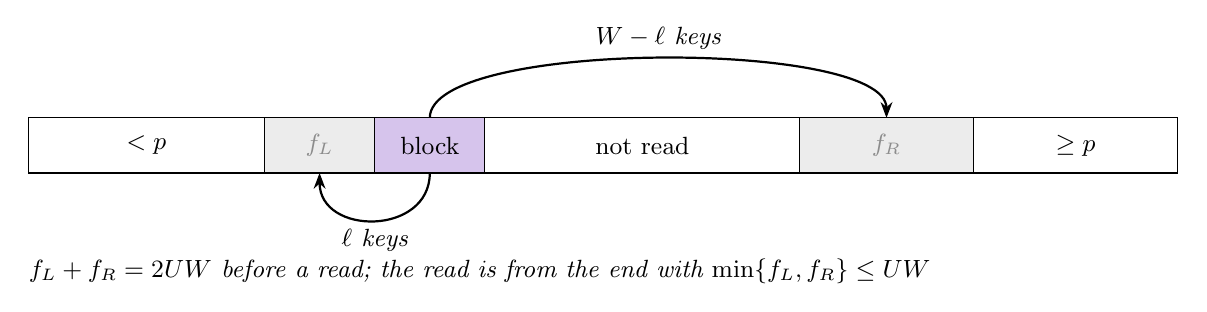
\begin{tikzpicture}[ads,
    seg/.style={cell,minimum height=7mm,font=\small},
    segf/.style={free,minimum height=7mm,font=\small},
    segt/.style={touched,minimum height=7mm,font=\small}]
  \node[seg,minimum width=30mm,anchor=west] (L) at (0,0) {$< p$};
  \node[segf,minimum width=14mm,anchor=west] (FL) at (L.east) {$f_L$};
  \node[segt,minimum width=14mm,anchor=west] (B) at (FL.east) {block};
  \node[seg,minimum width=40mm,anchor=west] (U) at (B.east) {not read};
  \node[segf,minimum width=22mm,anchor=west] (FR) at (U.east) {$f_R$};
  \node[seg,minimum width=26mm,anchor=west] (R) at (FR.east) {$\ge p$};
  \draw[ptr] (B.south) .. controls +(0,-8mm) and +(0,-8mm) .. node[var,below=1mm] {$\ell$ keys} (FL.south);
  \draw[ptr] (B.north) .. controls +(0,10mm) and +(0,10mm) .. node[var,above=1mm] {$W - \ell$ keys} (FR.north);
  \node[var,anchor=west] at (0,-16mm) {$f_L + f_R = 2 U W$ before a read; the read is from the end with $\min\{ f_L , f_R \} \le U W$};
\end{tikzpicture}
\end{document}
